\documentclass{article}
\usepackage{tikz}
\begin{document}
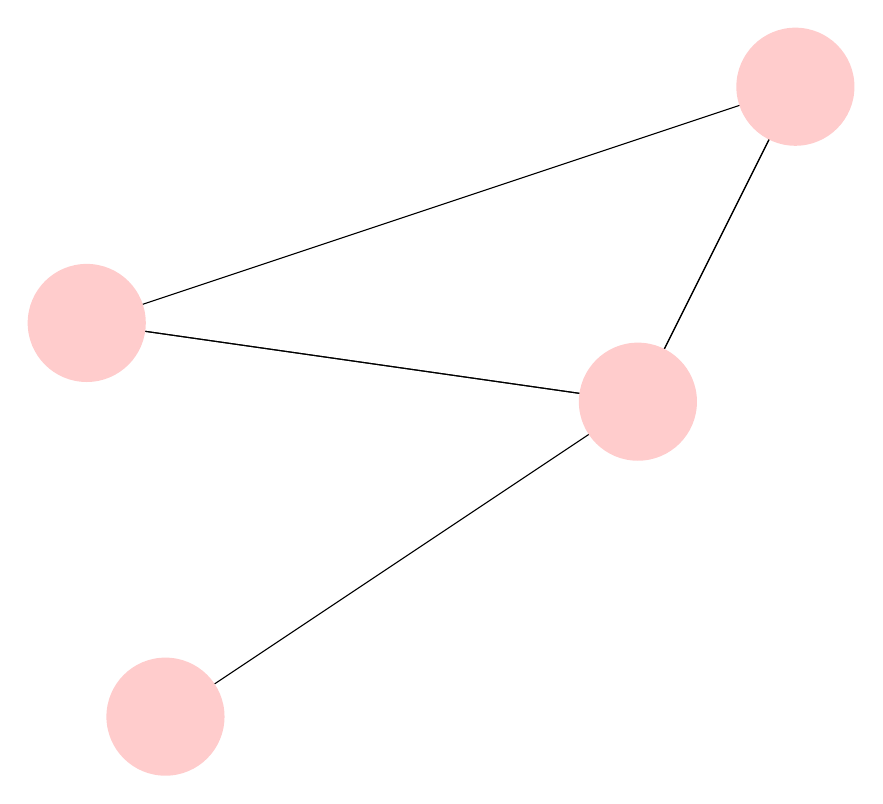
\begin{tikzpicture}
	\draw (3,-4) -- (10,-5);
	\draw (10,-5) -- (3,-4);
	\draw (10,-5) -- (4,-9);
	\draw (10,-5) -- (12,-1);
	\draw (12,-1) -- (10,-5);
	\draw (12,-1) -- (3,-4);
	\draw (3,-4) node[circle, fill=red!20, minimum size=1.5cm] {};
	\draw (10,-5) node[circle, fill=red!20, minimum size=1.5cm] {};
	\draw (4,-9) node[circle, fill=red!20, minimum size=1.5cm] {};
	\draw (12,-1) node[circle, fill=red!20, minimum size=1.5cm] {};
\end{tikzpicture}
\end{document}